\documentclass[border=3pt]{standalone}

%%Fonts
%\usepackage{fontspec}
%\setmainfont[Mapping=tex-text]{Times New Roman}
%\setmonofont[Mapping=tex-text]{JetBrains Mono}

%Drawing
\usepackage{tikz}

%Tikz Library
\usetikzlibrary{calc}

% Align text in the center of nodes
\tikzset{every text node part/.style={align=center}}

% Circuits
\usepackage{circuitikz}

% Colors
\usepackage{xcolor}
%
\definecolor{myblue}{HTML}{4698ED}
%
\def\muxcolor{orange!40}
\def\nonarchcolor{yellow!40}
\def\processingcolor{green!70!blue!30!}
\def\storagecolor{myblue!50}
\def\controlcolor{cyan!80!blue}

% Label
\tikzset{label_args/.style={
		font=\scriptsize\ttfamily,
	}
}

% FF size
\def\ffsize{2.2}
\def\ffwidth{1.3}

% CLK above components
\tikzset{clk/.pic = {
		\node[above] at (#1) {\scriptsize{CLK}};
	}
}

% Non-Architectural Flip Flop
\tikzset{non_arch_ff/.style={
	muxdemux,
	muxdemux def={
			Lh=\ffsize, Rh=\ffsize, w=\ffwidth, square pins=1,
			inset Lh=0, inset Rh=0, inset w=0,
			NL=1, NR=1, NB=0, NT=1,
		},
	muxdemux label ={
			cT1=1,
		},
	circuitikz/muxdemuxes/fill=\nonarchcolor,
    append after command={
			pic{clk=\tikzlastnode.tpin 1}
		},
	},
}

% Non-Architectural Flip Flop with We
\tikzset{non_arch_ff_we/.style={
	muxdemux,
	muxdemux def={
			Lh=\ffsize, Rh=\ffsize, w=\ffwidth, square pins=1,
			inset Lh=0, inset Rh=0, inset w=0,
			NL=1, NR=1, NB=1, NT=1,
		},
	muxdemux label ={
			cT1=1,
			B1=WE
		},
	circuitikz/muxdemuxes/fill=\nonarchcolor,
    append after command={
			pic{clk=\tikzlastnode.tpin 1}
		},
	},
}

% Architectural Flip Flop with We
\tikzset{ff_we/.style={
	muxdemux,
	muxdemux def={
			Lh=\ffsize, Rh=\ffsize, w=\ffwidth, square pins=1,
			inset Lh=0, inset Rh=0, inset w=0,
			NL=1, NR=1, NB=1, NT=1,
		},
	muxdemux label ={
			cT1=1,
			B1=WE,
		},
	circuitikz/muxdemuxes/fill=\storagecolor,
    append after command={
			pic{clk=\tikzlastnode.tpin 1}
		},
	},
}

% Instruction Memory
\tikzset{instr_mem/.style={
	muxdemux,
	muxdemux def={
			Lh=6, Rh=6, w=5, square pins=1,
			inset Lh=0, inset Rh=0, inset w=0,
			NL=2, NR=2, NB=0, NT=0,
		},
	muxdemux label ={
			L1=A,
			R1=RD,
		},
	draw only left pins={1},
	draw only right pins={1},
	circuitikz/muxdemuxes/fill=\storagecolor,
	circuitikz/muxdemux/inner label font=\scriptsize,
	},
}

% PC + 4
\tikzset{PC_4/.style={
	muxdemux,
	muxdemux def={
			Lh=3, Rh=1.4, w=1.5, square pins=1,
			inset Lh=1, inset Rh=0, inset w=0.75,
			NL=2, NR=1, NB=0, NT=0,
		},
	circuitikz/muxdemuxes/fill=\processingcolor
	},
}

% Register File
\tikzset{RF/.style={
	muxdemux,
	muxdemux def={
			Lh=9, Rh=9, w=5, square pins=1,
			inset Lh=0, inset Rh=0, inset w=0,
			NL=5, NR=2, NB=0, NT=5,
		},
	muxdemux label ={
			L1=A1, L2=A2, L3=A3, L4=R15, L5=WD3,
			R1=RD1, R2=RD2,
			cT2=1, T4=WE3
		},
	draw only top pins={2,4},
	circuitikz/muxdemuxes/fill=\storagecolor,
	circuitikz/muxdemux/inner label font=\scriptsize,
    append after command={
			pic{clk=\tikzlastnode.tpin 2}
		},
	},
}

% Extend Unit
\tikzset{extend/.style={
	muxdemux,
	muxdemux def={
			Lh=2, Rh=2.5, w=6, square pins=1,
			inset Lh=0, inset Rh=0, inset w=0,
			NL=1, NR=1, NB=0, NT=1,
		},
	circuitikz/muxdemuxes/fill=\processingcolor
	},
}

% MUX\documentclass[border=3pt]{standalone}
\tikzset{mux2to1/.style={
	muxdemux,
	muxdemux def={
			Lh=2, Rh=1.5, w=0.8, square pins=1,
			inset Lh=0, inset Rh=0, inset w=0,
			NL=2, NR=1, NB=0, NT=1,
		},
	muxdemux label ={
			L1=0, L2=1,
		},
	circuitikz/muxdemuxes/fill=\muxcolor,
	circuitikz/muxdemux/inner label font=\small,
	},
}
\tikzset{mux2to1_reverse/.style={
	muxdemux,
	muxdemux def={
			Lh=2, Rh=1.5, w=0.8, square pins=1,
			inset Lh=0, inset Rh=0, inset w=0,
			NL=2, NR=1, NB=0, NT=1,
		},
	muxdemux label ={
			L1=1, L2=0,
		},
	circuitikz/muxdemuxes/fill=\muxcolor,
	circuitikz/muxdemux/inner label font=\small,
	},
}

% ALU
\tikzset{ALU/.style={
	muxdemux,
	muxdemux def={
			Lh=8, Rh=3.5, w=2.5, square pins=1,
			inset Lh=2, inset Rh=0, inset w=1.2,
			NL=2, NR=1, NB=0, NT=3,
		},
	circuitikz/muxdemuxes/fill=\processingcolor,
	external pins width=1,
	},
}

% Data Memory
\tikzset{data_mem/.style={
	muxdemux,
	muxdemux def={
			Lh=8, Rh=8, w=4, square pins=1,
			inset Lh=0, inset Rh=0, inset w=0,
			NL=3, NR=3, NB=0, NT=6,
		},
	muxdemux label ={
			L1=A, L3=WD,
			R3=RD,
			cT2=1, T5=WE,
		},
	draw only left pins={1,3},
	draw only right pins={3},
	draw only top pins={2,5},
	circuitikz/muxdemuxes/fill=\storagecolor,
	circuitikz/muxdemux/inner label font=\scriptsize,
    append after command={
			pic{clk=\tikzlastnode.tpin 2}
		},
	},
}

% MUX 3 to 1
\tikzset{mux3to1/.style={
	muxdemux,
	muxdemux def={
			Lh=2, Rh=2.4, w=0.8, square pins=1,
			inset Lh=0, inset Rh=0, inset w=0,
			NL=1, NR=3, NB=0, NT=1,
		},
	muxdemux label ={
			R1=00, R2=01, R3=10,
		},
	circuitikz/muxdemuxes/fill=\muxcolor,
	circuitikz/muxdemux/inner label font=\scriptsize,
	},
}

% MUX\documentclass[border=3pt]{standalone}
\tikzset{mux2to1_leftsided/.style={
	muxdemux,
	muxdemux def={
			Lh=2.4, Rh=3, w=0.8, square pins=1,
			inset Lh=0, inset Rh=0, inset w=0,
			NL=1, NR=2, NB=0, NT=1,
		},
	muxdemux label ={
			R1=0, R2=1,
		},
	circuitikz/muxdemuxes/fill=\muxcolor,
	circuitikz/muxdemux/inner label font=\small,
	},
}

% Control Signal
\newcommand{\control}[3]{
	\node[#3] at (#2) {\ttfamily\scriptsize\color{\controlcolor}#1};
}

\begin{document}
	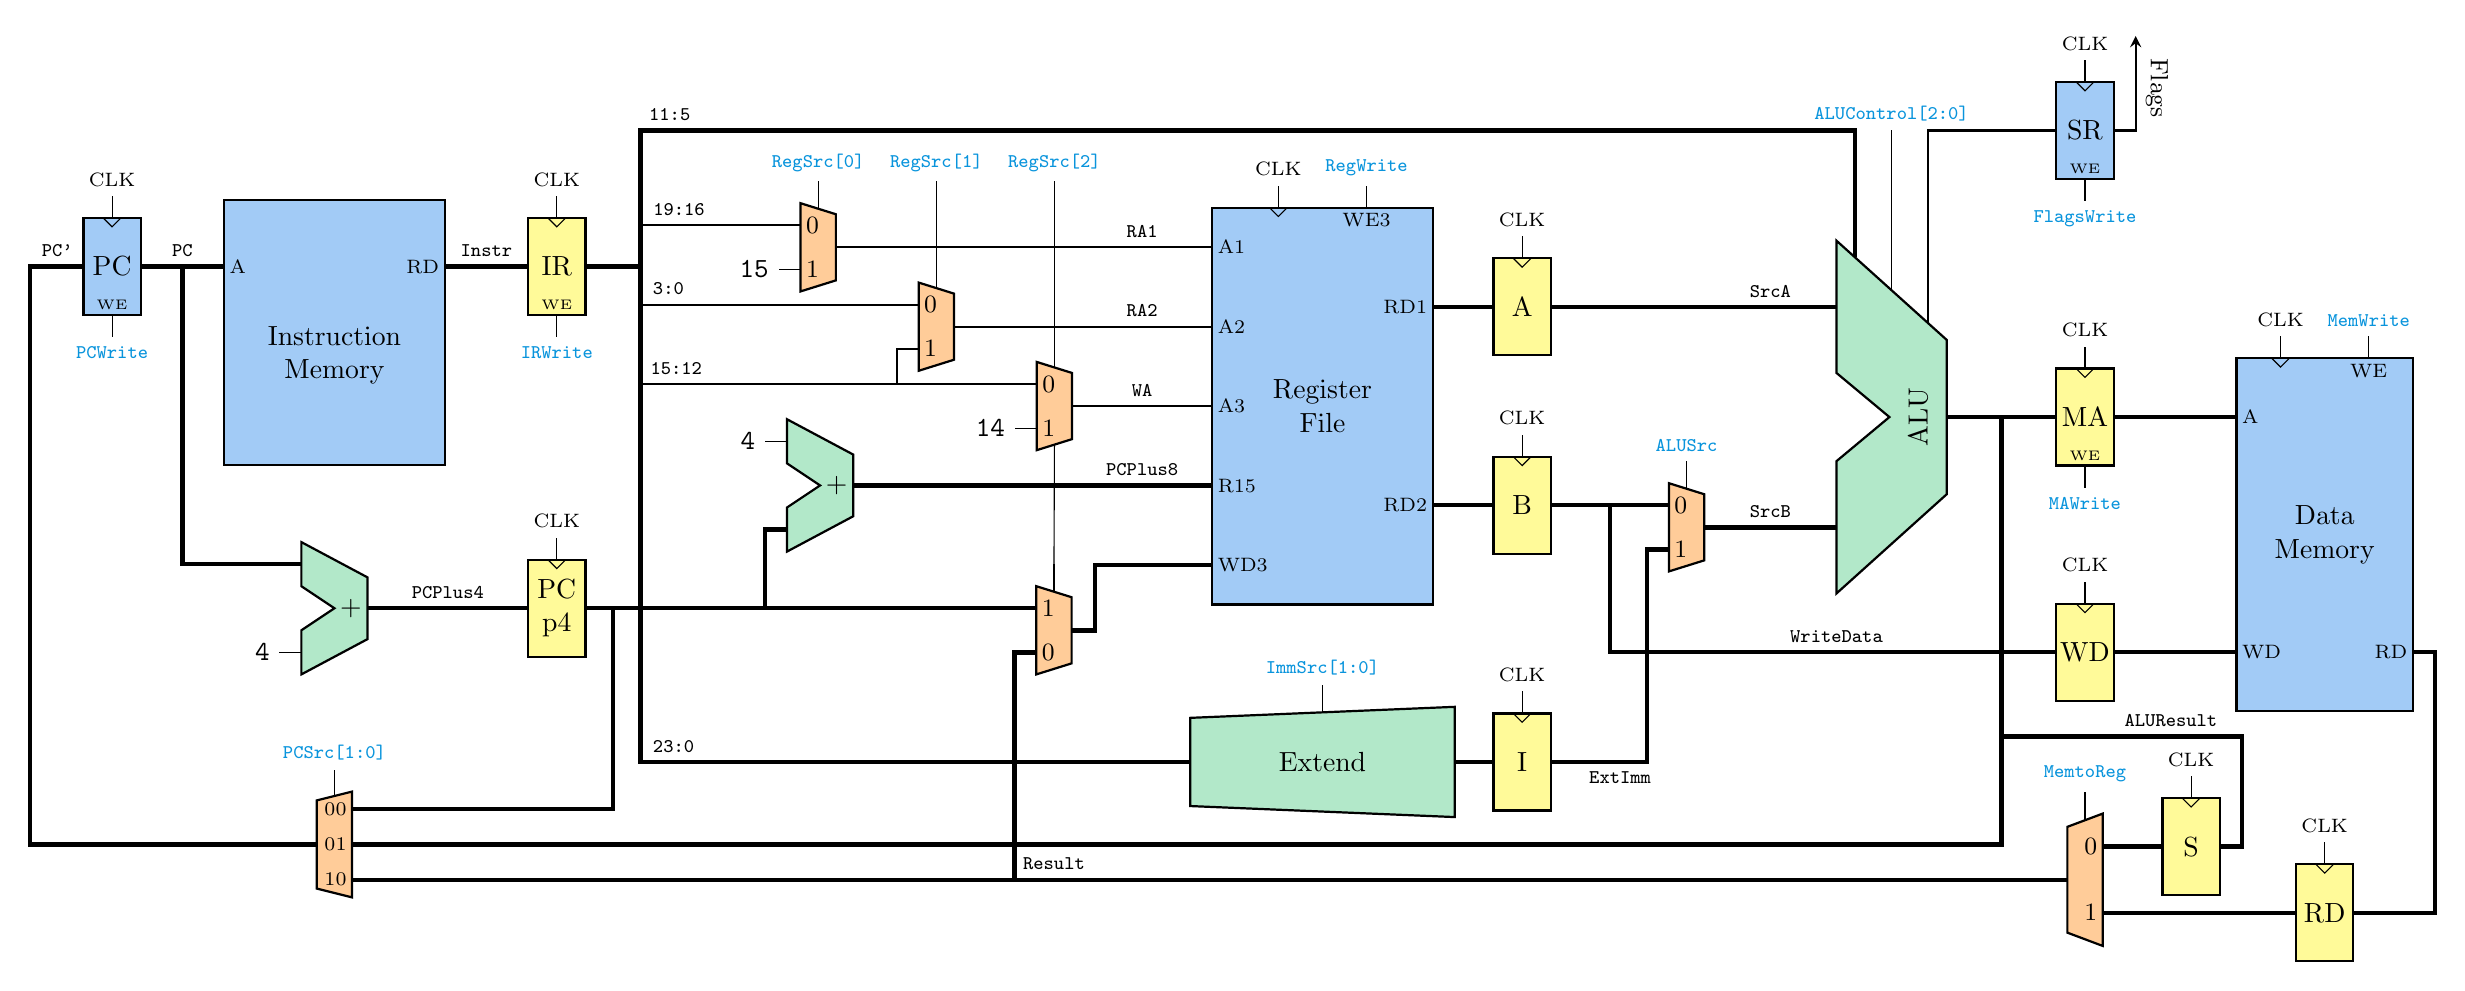
\begin{tikzpicture}
		%%%% Components %%%%
		
		% PC
		\node[ff_we] (PC) 
			 at (0,0) {PC};
			 
		% Instruction Memory
		\node[instr_mem, anchor=lpin 1, xshift=0.5cm] (instr_mem)
			 at (PC.rpin 1) {\\[4mm]Instruction\\Memory};
			 
		% IR
		\node[non_arch_ff_we, anchor=lpin 1, xshift=0.5cm] (IR) 
			 at (instr_mem.rpin 1) {IR};			 
			 
		% PC + 4
		\node[PC_4] (PCPlus4) 
   			 at ($(instr_mem.center) + (0,-3.5)$) {+};			
   			 
		% PC p4
		\node[non_arch_ff] (PC_p4) 
			 at (IR.bpin 1|-PCPlus4) {PC\\p4};
			 
		% PC + 8
		\node[PC_4, anchor=lpin 2, shift={(2cm,1cm)}] (PCPlus8) 
   			 at (PC_p4.rpin 1) {+};
   			 
   		% Register File
		\node[RF, anchor=lpin 4, xshift=4cm] (RF) 
   			 at (PCPlus8.rpin 1) {Register\\File};	
   			 
   		% Extend Unit
   		\node[extend, yshift=-2cm] (Extend)
   			 at (RF.bottom) {Extend};
   			 
   		% MUX A1
   		\node[mux2to1, anchor=brpin 1, xshift=-4.5cm] (mux2to1_A1)
   			 at (RF.lpin 1) {};
   			 
   		% MUX A2
   		\node[mux2to1, anchor=brpin 1, xshift=-3cm] (mux2to1_A2)
   			 at (RF.lpin 2) {};
   			 
   		% MUX A3
   		\node[mux2to1, anchor=brpin 1, xshift=-1.5cm] (mux2to1_A3)
   			 at (RF.lpin 3) {};
   			 
   		% MUX WD3
   		\node[mux2to1_reverse, anchor=blpin 1, xshift=-0.23cm] (mux2to1_WD3)
   			 at (PC_p4.brpin 1-|mux2to1_A3) {};
   			 
		% A
		\node[non_arch_ff, anchor=rpin 1, xshift=1.5cm] (A) 
			 at (RF.rpin 1) {A};	
			 
		% B
		\node[non_arch_ff, anchor=rpin 1, xshift=1.5cm] (B) 
			 at (RF.rpin 2) {B};	
			 
		% I
		\node[non_arch_ff] (I) 
			 at (Extend.rpin 1-|A) {I};	
			 
   		% MUX B
   		\node[mux2to1, anchor=blpin 1, xshift=1.5cm] (mux2to1_B)
   			 at (B.brpin 1) {};
   			 
		% ALU
		\node[ALU, anchor=lpin 2, xshift=0cm] (ALU) 
   			 at (mux2to1_B.rpin 1) {\rotatebox{90}{ALU}};
			 
		% MA
		\node[non_arch_ff_we, anchor=rpin 1, xshift=1cm] (MA) 
			 at (ALU.rpin 1) {MA};	
			 
		% Status Register
		\node[ff_we] (SR) 
			 at (MA|-ALU.tpin 3) {SR};
		
		% Data Memory
		\node[data_mem, anchor=lpin 1, xshift=1cm] (data_mem)
			 at (MA.rpin 1) {Data\\Memory};
			 
		% WD
		\node[non_arch_ff, anchor=rpin 1, xshift=-1cm] (WD) 
			 at (data_mem.lpin 3) {WD};	
		
		% MUX 3 to 1	 
		\node[mux3to1, yshift=-3cm] (mux3to1)
			 at (PCPlus4) {};
		
		% MUX\documentclass[border=3pt]{standalone}
		\node[mux2to1_leftsided] (mux2to1_leftsided)
			 at (mux3to1.rpin 3-|WD) {};
			 
		% S
		\node[non_arch_ff, anchor=lpin 1, xshift=0.2cm] (S)
			 at (mux2to1_leftsided.rpin 1) {S};

		% RD
		\node[non_arch_ff] (RD)
			 at (mux2to1_leftsided.rpin 2-|data_mem) {RD};
		
		%%%% Connections %%%%
		
		% Buses of 32 bits
		\draw[ultra thick] 
			 (PC.brpin 1) -- (instr_mem.blpin 1)
			 %
			 (instr_mem.brpin 1) -- (IR.blpin 1)
			 %
			 (PCPlus4.blpin 1) -| ($(PC.rpin 1)!0.5!(instr_mem.lpin 1)$)
	  		 (PCPlus4.brpin 1) -- (PC_p4.blpin 1)
			 (PC_p4.brpin 1) -| (PCPlus8.lpin 2) -- (PCPlus8.blpin 2)
			 %
			 (PCPlus8.brpin 1) -- (RF.blpin 4)
			 %
			 (IR.brpin 1) -- +(0.7,0) coordinate (ir_tmp)
			 			  -- (ir_tmp|-ALU.tpin 1)
			 			  -- (ir_tmp|-Extend.lpin 1)
			 			  -- (Extend.blpin 1)
			 %
  			 (mux2to1_WD3.brpin 1) -- ++(0.3,0) |- (RF.blpin 5)
			 (mux2to1_WD3.blpin 1) -- (PC_p4.brpin 1)
  			 (mux2to1_WD3.blpin 2) -- (mux2to1_WD3.lpin 2) 
  			 					   -- (mux2to1_WD3.lpin 2|-mux3to1.rpin 3)
  			 %
  			 (RF.brpin 1) -- (A.blpin 1)
  			 (RF.brpin 2) -- (B.blpin 1)
  			 %
  			 (Extend.brpin 1) -- (I.blpin 1)
  			 %
  			 (B.brpin 1) -- (mux2to1_B.blpin 1)
  			 (I.brpin 1) -| (mux2to1_B.lpin 2) -- (mux2to1_B.blpin 2)
  			 %
  			 (ALU.blpin 1) -- (A.brpin 1)
  			 (ALU.blpin 2) -- (mux2to1_B.brpin 1)
  			 %
  			 (ALU.brpin 1) -- (MA.blpin 1)
  			 %
  			 (MA.brpin 1) -- (data_mem.blpin 1)
  			 %
  			 (data_mem.blpin 3) -- (WD.brpin 1)
  			 (data_mem.brpin 3) -- (data_mem.rpin 3) |- (RD.rpin 1) -- (RD.brpin 1)
  			 %
  			 (WD.blpin 1) -| ($(B.brpin 1)!0.5!(mux2to1_B.blpin 1)$)
  			 %
  			 (mux3to1.blpin 1) -| ($(PC.lpin 1)+(-0.4,0)$) -- (PC.blpin 1)
  			 (mux3to1.brpin 1) -| ($(PC_p4.brpin 1)+(0.35,0)$)
  			 (mux3to1.brpin 2) -| ($(ALU.brpin 1)!0.5!(MA.blpin 1)$) coordinate (ALU_tmp)
  			 (mux3to1.brpin 3) -- (mux2to1_leftsided.blpin 1)
  			 %
  			 (mux2to1_leftsided.brpin 1) -- (S.blpin 1)
  			 (mux2to1_leftsided.brpin 2) -- (RD.blpin 1)
  			 %
  			 (S.brpin 1) -- (S.rpin 1) -- ++(0,1.4cm) coordinate (S_tmp)
  			             -- (S_tmp-|ALU_tmp)
			 %
			 (ALU.btpin 1) -- (ALU.tpin 1) |- (ALU.tpin 1-|ir_tmp) -- (ir_tmp);

		% Smaller Buses			 			  
		\draw[thick]
			 (mux2to1_A1.brpin 1) -- (RF.blpin 1)
			 (mux2to1_A1.blpin 1) -- (mux2to1_A1.blpin 1-|ir_tmp)
			 %
 			 (mux2to1_A3.brpin 1) -- (RF.blpin 3)
			 (mux2to1_A3.blpin 1) -- (mux2to1_A3.blpin 1-|ir_tmp)
			 %
 			 (mux2to1_A2.brpin 1) -- (RF.blpin 2)
			 (mux2to1_A2.blpin 1) -- (mux2to1_A2.blpin 1-|ir_tmp)
			 (mux2to1_A2.blpin 2) -| (mux2to1_A2.lpin 1|-mux2to1_A3.blpin 1)
			 %
			 (ALU.btpin 3) -- (ALU.tpin 3) -- (SR.blpin 1)
			 [-stealth] (SR.brpin 1) -- (SR.rpin 1) 
			 			 -- +(0,1.2) node[right,pos=0.45] {\rotatebox{-90}{\small{Flags}}};
		
		%%%% Control %%%%
		\control{PCWrite}{PC.bpin 1}{below};
		%
		\control{IRWrite}{IR.bpin 1}{below};
		%
		\control{ImmSrc[1:0]}{Extend.tpin 1}{above};
		%
		\control{RegSrc[0]}{mux2to1_A1.tpin 1}{above};
		%
		\draw (mux2to1_A2.tpin 1) -- (mux2to1_A2.tpin 1|-mux2to1_A1.tpin 1)
			  coordinate (control_mux2to1_A1);
		\control{RegSrc[1]}{control_mux2to1_A1}{above};		
		%
		\draw (mux2to1_A3.tpin 1) -- (mux2to1_A3.tpin 1|-mux2to1_A1.tpin 1)
			  coordinate (control_mux2to1_A3);
		\control{RegSrc[2]}{control_mux2to1_A3}{above};	
		%
		\draw (mux2to1_WD3.tpin 1) -- (mux2to1_A3.bottom);
		%
		\control{RegWrite}{RF.tpin 4}{above};
		%
		\control{ALUSrc}{mux2to1_B.tpin 1}{above};
		%
		\control{ALUControl[2:0]}{ALU.tpin 2}{above};
		%
		\control{FlagsWrite}{SR.bpin 1}{below};
		%
		\control{MAWrite}{MA.bpin 1}{below};
		%
		\control{MemWrite}{data_mem.tpin 5}{above};
		%
		\control{PCSrc[1:0]}{mux3to1.tpin 1}{above};
		%
		\control{MemtoReg}{mux2to1_leftsided.tpin 1}{above};
		
		%%%% Inputs %%%%
		\node[left] at (PCPlus4.lpin 2) {\ttfamily4};
		%
		\node[left] at (PCPlus8.lpin 1) {\ttfamily4};
		%
		\node[left] at (mux2to1_A1.lpin 2) {\ttfamily15};
		%
		\node[left] at (mux2to1_A3.lpin 2) {\ttfamily14};
		
		%%%% Instruction Bits %%%%
		\node[above] at 
			 ($(mux2to1_A1.blpin 1-|ir_tmp)!0.24!(mux2to1_A1.blpin 1)$) 
			 {\scriptsize\ttfamily19:16};
		%
		\node[above] at 
			 ($(mux2to1_A2.blpin 1-|ir_tmp)!0.1!(mux2to1_A2.blpin 1)$) 
			 {\scriptsize\ttfamily3:0};
		%
		\node[above] at 
			 ($(mux2to1_A3.blpin 1-|ir_tmp)!0.09!(mux2to1_A3.blpin 1)$) 
			 {\scriptsize\ttfamily15:12};
		%
		\node[above] at 
			 ($(Extend.blpin 1-|ir_tmp)!0.06!(Extend.blpin 1)$) 
			 {\scriptsize\ttfamily23:0};
		%
		\node[above] at 
			 ($(ALU.tpin 1-|ir_tmp)!0.024!(ALU.tpin 1)$) 
			 {\scriptsize\ttfamily11:5};
			 
		%%%% Labels %%%%
		\node[label_args, above, xshift=-1.5pt] at 
			 (PC.lpin 1) {PC'};
		\node[label_args, above] at 
			 ($(PC.rpin 1)!0.5!(instr_mem.lpin 1)$) {PC};
		\node[label_args, above] at 
			 ($(instr_mem.rpin 1)!0.5!(IR.lpin 1)$) {Instr};
		\node[label_args, above] at 
			 ($(PCPlus4.rpin 1)!0.5!(PC_p4.lpin 1)$) {PCPlus4};
		\node[label_args, below, xshift=0.6cm] at 
			 (I.rpin 1) {ExtImm};
		\node[label_args, above] (SrcB) at 
			 ($(mux2to1_B.brpin 1)!0.5!(ALU.blpin 2)$) {SrcB};
		\node[label_args, above] at 
			 (A-|SrcB) {SrcA};
		\node[label_args, above] at 
			 (WD.lpin 1-|ALU.blpin 2) {WriteData};
		\node[label_args, above, xshift=-0.9cm] at 
			 (S_tmp) {ALUResult};
		\node[label_args, above] at 
			 (mux2to1_leftsided-|mux2to1_WD3) {Result};
		\node[label_args, above] (WA) at 
			 ($(mux2to1_A3.rpin 1)!0.5!(RF.lpin 3)$) {WA};
		\node[label_args, above] at 
			 (WA|-mux2to1_A1) {RA1};
		\node[label_args, above] at 
			 (WA|-mux2to1_A2) {RA2};
		\node[label_args, above] at 
			 (WA|-PCPlus8) {PCPlus8};
	\end{tikzpicture}
\end{document}